\documentclass[]{article}
\usepackage[left=1in,top=1in,right=1in,bottom=1in]{geometry}


%%%% more monte %%%%
% thispagestyle{empty}
% https://stackoverflow.com/questions/2166557/how-to-hide-the-page-number-in-latex-on-first-page-of-a-chapter
\usepackage{color}
% \usepackage[table]{xcolor} % are they using color?

% \definecolor{WSU.crimson}{HTML}{981e32}
% \definecolor{WSU.gray}{HTML}{5e6a71}

% \definecolor{shadecolor}{RGB}{248,248,248}
\definecolor{WSU.crimson}{RGB}{152,30,50} % use http://colors.mshaffer.com to convert from 981e32
\definecolor{WSU.gray}{RGB}{94,106,113}

%%%%%%%%%%%%%%%%%%%%%%%%%%%%

\newcommand*{\authorfont}{\fontfamily{phv}\selectfont}
\usepackage{lmodern}


  \usepackage[T1]{fontenc}
  \usepackage[utf8]{inputenc}




\usepackage{abstract}
\renewcommand{\abstractname}{}    % clear the title
\renewcommand{\absnamepos}{empty} % originally center

\renewenvironment{abstract}
 {{%
    \setlength{\leftmargin}{0mm}
    \setlength{\rightmargin}{\leftmargin}%
  }%
  \relax}
 {\endlist}

\makeatletter
\def\@maketitle{%
  \pagestyle{empty}
  \newpage
%  \null
%  \vskip 2em%
%  \begin{center}%
  \let \footnote \thanks
    {\fontsize{18}{20}\selectfont\raggedright  \setlength{\parindent}{0pt} \@title \par}%
}
%\fi
\makeatother









\title{\textbf{\textcolor{WSU.crimson}{Will v.
Denzel}} \newline \textbf{\textcolor{WSU.gray}{An Investigation on who
is Better}}  }
 

%  

% \author{ \Large true \hfill \normalsize \emph{} }
\author{\Large Nathan
Shine\vspace{0.05in} \newline\normalsize\emph{Washington State
University}  }


\date{December 14, 2020}
\setcounter{secnumdepth}{3}

\usepackage{titlesec}
% See the link above: KOMA classes are not compatible with titlesec any more. Sorry.
% https://github.com/jbezos/titlesec/issues/11
\titleformat*{\section}{\bfseries}
\titleformat*{\subsection}{\bfseries\itshape}
\titleformat*{\subsubsection}{\itshape}
\titleformat*{\paragraph}{\itshape}
\titleformat*{\subparagraph}{\itshape}

% https://code.usgs.gov/usgs/norock/irvine_k/ip-092225/


%\titleformat*{\section}{\normalsize\bfseries}
%\titleformat*{\subsection}{\normalsize\itshape}
%\titleformat*{\subsubsection}{\normalsize\itshape}
%\titleformat*{\paragraph}{\normalsize\itshape}
%\titleformat*{\subparagraph}{\normalsize\itshape}

% https://tex.stackexchange.com/questions/233866/one-column-multicol-environment#233904
\usepackage{environ}
\NewEnviron{auxmulticols}[1]{%
  \ifnum#1<2\relax% Fewer than 2 columns
    %\vspace{-\baselineskip}% Possible vertical correction
    \BODY
  \else% More than 1 column
    \begin{multicols}{#1}
      \BODY
    \end{multicols}%
  \fi
}





\usepackage{natbib}
\setcitestyle{aysep={}} %% no year, comma just year
% \usepackage[numbers]{natbib}
\bibliographystyle{./../../biblio/ormsv080.bst}



\usepackage[strings]{underscore} % protect underscores in most circumstances




\newtheorem{hypothesis}{Hypothesis}
\usepackage{setspace}


%%%%%%%%%%%%%%%%%%%%%%%%%%%%%%%%%%%%%%%%%%%%%%%%%%%%%
%%% MONTE ADDS %%%

\usepackage{fancyhdr} % fancy header 
\usepackage{lastpage} % last page 

\usepackage{multicol}


\usepackage{etoolbox}
\AtBeginEnvironment{quote}{\singlespacing\small}
% https://tex.stackexchange.com/questions/325695/how-to-style-blockquote


\usepackage{soul}			%% allows strike-through
\usepackage{url}			%% fixes underscores in urls
\usepackage{csquotes}		%% allows \textquote in references
\usepackage{rotating}		%% allows table and box rotation
\usepackage{caption}		%% customize caption information
\usepackage{booktabs}		%% enhance table/tabular environment
\usepackage{tabularx}		%% width attributes updates tabular
\usepackage{enumerate}		%% special item environment
\usepackage{enumitem}		%% special item environment

\usepackage{lineno}		%% allows linenumbers for editing using \linenumbers
\usepackage{hanging}


\usepackage{mathtools}  	%% also loads amsmath
\usepackage{bm}		%% bold-math
\usepackage{scalerel}	%% scale one element (make one beta bigger font)

\newcommand{\gFrac}[2]{ \genfrac{}{}{0pt}{1}{{#1}}{#2} }

\newcommand{\betaSH}[3]{  \gFrac{\text{\tiny #1}}{{\text{\tiny #2}}}\hat{\beta}_{\text{#3}}   }
\newcommand{\betaSB}[3]{              ^{\text{#1}} _{\text{#2}} \bm{\beta} _{\text{#3}}                   }  %% bold
\newcommand{\bigEQ}{  \scaleobj{1.5}{{\ }= } }
\newcommand{\bigP}[1]{  \scaleobj{1.5}{#1 } }





\usepackage{endnotes}  % he already does this ...
\renewcommand{\enotesize}{\normalsize}
% https://tex.stackexchange.com/questions/99984/endnotes-do-not-be-superscript-and-add-a-space
\renewcommand\makeenmark{\textsuperscript{[\theenmark]}} % in brackets %
% https://tex.stackexchange.com/questions/31574/how-to-control-the-indent-in-endnotes
\patchcmd{\enoteformat}{1.8em}{0pt}{}{}

\patchcmd{\theendnotes}
  {\makeatletter}
  {\makeatletter\renewcommand\makeenmark{\textbf{[\theenmark]} }}
  {}{}



% https://tex.stackexchange.com/questions/141906/configuring-footnote-position-and-spacing

\addtolength{\footnotesep}{5mm} % change to 1mm

\renewcommand{\thefootnote}{\textbf{\arabic{footnote}}}
\let\footnote=\endnote
%\renewcommand*{\theendnote}{\alph{endnote}}
%\renewcommand{\theendnote}{\textbf{\arabic{endnote}}}


\renewcommand*{\notesname}{ENDNOTES}

\makeatletter
\def\enoteheading{\section*{\notesname
  \@mkboth{\MakeUppercase{\notesname}}{\MakeUppercase{\notesname}}}%
  \mbox{}\par\vskip-2.3\baselineskip\noindent\rule{.5\textwidth}{0.4pt}\par\vskip\baselineskip}
\makeatother


\renewcommand*{\contentsname}{TABLE OF CONTENTS}

\renewcommand*{\refname}{REFERENCES}


%\usepackage{subfigure}
\usepackage{subcaption}

\captionsetup{labelfont=bf}  % Make Table / Figure bold

%%% you could add elements here ... monte says .... %%%
%\usepackage{mypackageForCapitalH}


%%%%%%%%%%%%%%%%%%%%%%%%%%%%%%%%%%%%%%%%%%%%%%%%%%%%%

% set default figure placement to htbp
\makeatletter
\def\fps@figure{htbp}
\makeatother


% move the hyperref stuff down here, after header-includes, to allow for - \usepackage{hyperref}

\makeatletter
\@ifpackageloaded{hyperref}{}{%
\ifxetex
  \PassOptionsToPackage{hyphens}{url}\usepackage[setpagesize=false, % page size defined by xetex
              unicode=false, % unicode breaks when used with xetex
              xetex]{hyperref}
\else
  \PassOptionsToPackage{hyphens}{url}\usepackage[draft,unicode=true]{hyperref}
\fi
}

\@ifpackageloaded{color}{
    \PassOptionsToPackage{usenames,dvipsnames}{color}
}{%
    \usepackage[usenames,dvipsnames]{color}
}
\makeatother
\hypersetup{breaklinks=true,
            bookmarks=true,
            pdfauthor={Nathan Shine (Washington State University)},
             pdfkeywords = {t-tests; proportions; data collection;
correlation investigation},  
            pdftitle={Will v. Denzel: An Investigation on who is
Better},
            colorlinks=true,
            citecolor=blue,
            urlcolor=blue,
            linkcolor=magenta,
            pdfborder={0 0 0}}
\urlstyle{same}  % don't use monospace font for urls

% Add an option for endnotes. -----

%
% add tightlist ----------
\providecommand{\tightlist}{%
\setlength{\itemsep}{0pt}\setlength{\parskip}{0pt}}

% add some other packages ----------

% \usepackage{multicol}
% This should regulate where figures float
% See: https://tex.stackexchange.com/questions/2275/keeping-tables-figures-close-to-where-they-are-mentioned
\usepackage[section]{placeins}



\pagestyle{fancy}   
\lhead{\textcolor{WSU.crimson}{\textbf{ Will v. Denzel }}}
\chead{}
\rhead{\textcolor{WSU.gray}{\textbf{  Page\ \thepage\ of\ \protect\pageref{LastPage} }}}
\lfoot{}
\cfoot{}
\rfoot{}


\begin{document}
	
% \pagenumbering{arabic}% resets `page` counter to 1 
%    

% \maketitle

{% \usefont{T1}{pnc}{m}{n}
\setlength{\parindent}{0pt}
\thispagestyle{plain}
{\fontsize{18}{20}\selectfont\raggedright 
\maketitle  % title \par  

}

{
   \vskip 13.5pt\relax \normalsize\fontsize{11}{12} 
   
\textbf{\authorfont Nathan Shine} \hskip 15pt \emph{\small Washington
State University}   

}

}








\begin{abstract}

    \hbox{\vrule height .2pt width 39.14pc}

    \vskip 8.5pt % \small 

\noindent In this article we abstract

\noindent Abstract\vspace{0.25in}


\vskip 8.5pt \noindent \textbf{\underline{Keywords}:} t-tests;
proportions; data collection; correlation investigation \par

    




    
    \hbox{\vrule height .2pt width 39.14pc}
    \vskip 5pt 
    \hfill \textbf{\textcolor{WSU.gray}{ December 14, 2020 } }
    \vskip 5pt 
    
\end{abstract}


\vskip -8.5pt



 % removetitleabstract

\noindent  

\section{Introduction}
\label{sec:intro}

\begin{quote}
“You’ll never see a U-Haul behind a hearse. … Now, I’ve been blessed to make hundreds of millions of dollars in my life. I can’t take it with me, and neither can you. It’s not how much you have but what you do with what you have.” – Denzel Washington
\end{quote}

Will Smith and Denzel Washington are two of the most prominent movie
stars in the business today, though they have very different stories.
Will Smith burst onto the scene as ``The Fresh Prince'' in the rap duo
group ``DJ Jazzy Jeff \& The Fresh Prince,'' winning his first Grammy
award when he was just 20. Smith later starred in the TV show
\emph{The Fresh Prince of Bel-Air} from 1990-1996. After this period he
started to achieve a wide amount of commercial success from movies like
\emph{Bad Boys}, \emph{Independence Day}, and \emph{Men in Black}.
Denzel began his career as a theater actor in Maryland before he
received a regular role as Dr.~Chandler on TV show \emph{St. Elsewhere}.
Denzel then began to branch out into feature films receiving his first
Oscar nomination in the movie \emph{Cry Freedom} (1987) and his first
win (Best Supporting Actor) in the movie \emph{Glory} (1990) shortly
afterward. It is without question that both actors have achieved a
monumental amount of success in their careers, but the question remains:
Which one of the two is better?

I will explore the answer to this question by examining the differences
between the two. Which types of movies they are successful in, comparing
their awards, looking at the money their movies have made, and
investigating the impact they have made on the movie scene each year.
These are pieces of the puzzle that I will show below in this report.

\newpage
\section{Commercial Impact on Industry}

The movie business has enjoyed incredible commercial success growing
since the latter half of the 20th century. When controlling for
inflation we can see that the movie business has enjoyed a fairly linear
growth from the 1950s until the early 2000s where it has since
stagnated.

\begin{figure}
  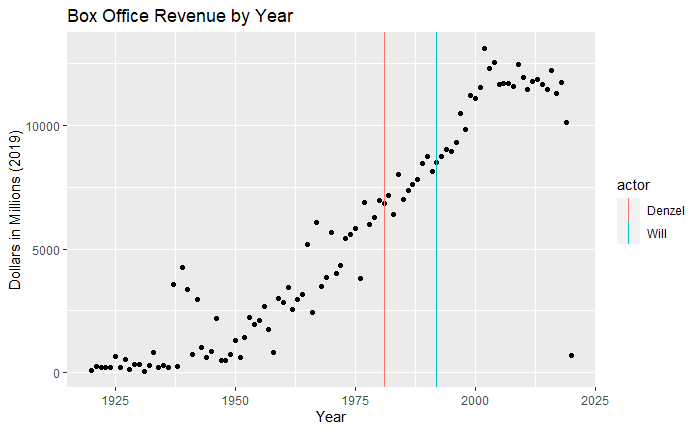
\includegraphics[clip,scale=0.5]{plots/revenue_by_year.png}
  \caption{\textbf{Movie Commercial Growth}}
  \label{fig:yearly-rev}
\end{figure}

As can be seen in figure \ref{fig:yearly-rev} above, Denzel's career
began about ten years before Will's, and in this period he has seen more
commercial growth of the industry than his peer. We shall now examine
the impact of each actor's movies on the commercial success of each
year.

\begin{figure}[!ht]
    \begin{subfigure}[h]{0.5\textwidth}
    \centering
    %  trim={<left> <lower> <right> <upper>}
    % https://shantoroy.com/latex/add-subfig-in-latex/
            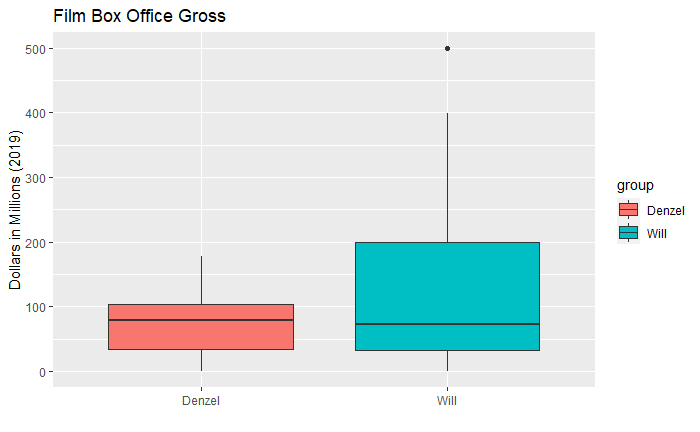
\includegraphics[clip,scale=0.4]{plots/gross_dist.png}
        \caption{ Movie Revenue Distribution}
        \label{fig:rev-dist-plot}
    \end{subfigure}
    \begin{subfigure}[h]{0.5\textwidth}
    \centering
        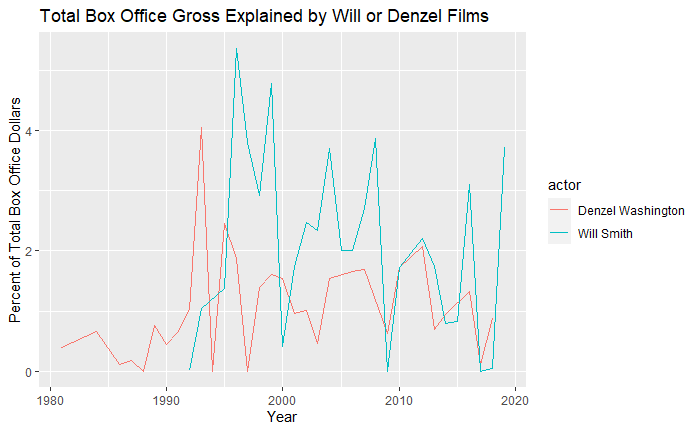
\includegraphics[clip,scale=0.4]{plots/total_gross.png}
            \caption{Proportional Movie Revenue}
        \label{fig:prop-gross-plot}
    \end{subfigure}
    \vspace{2.5mm}
    \hrule
    \vspace{2.5mm}
        \caption{\textbf{ Commercial Impact } }
        \label{fig:ce-plot}
\end{figure}

Above in figure \ref{fig:prop-gross-plot}, is shown the amount of the
total box office revenue explained by each actor. For each year, and for
each actor, I found the proportion of their movie revenues to total
movie revenues for that year. As we can see Will Smith has much higher
peaks for his movies. This tells us that in these years more people went
to see his movies in the theaters. When researching for this project, I
learned that Will Smith was called ``Mr.~July'' around this time,
because it seemed like every summer he would release a big movie that
people would go see.

In contrast, Denzel Washington's movies don't explain nearly as much of
the total revenue as Will's do. However, whereas Will's movies seem to
be less commercially dominant overtime, Denzel's movies releases have
shown relative stability for the last two decades. There is one major
spike for Denzel, which is in the year 1995 when he released the highly
successful \emph{Crimson Tide}, along with \emph{Virtuosity}, and
\emph{Devil in a Blue Dress}.

The wide difference in commercial impact from figure
\ref{fig:prop-gross-plot} may suggest that Denzel Washington's movies
are not met with great commercial success. On the contrary, from figure
\ref{fig:rev-dist-plot} we can see that while Will Smith's movies have a
higher revenue ceiling, the average Denzel Washington movie is more
commercially successful than the average Will Smith one! It may also
surprise one to learn that despite having about a ten year head start on
Will, Denzel has only made 61 movies compared to Will's 111. From this
high number of movies one can see why there is a much greater
variability in the commercial success of the works of Will Smith.

\section{Movies Types}

In this section, I will delve deeper into the types of movies that Will
and Denzel make. Besides being very different personalities, Will and
Denzel produce films that differ a lot from each other. These
differences come in the case of genre and the target audience.

\begin{figure}[!ht]
  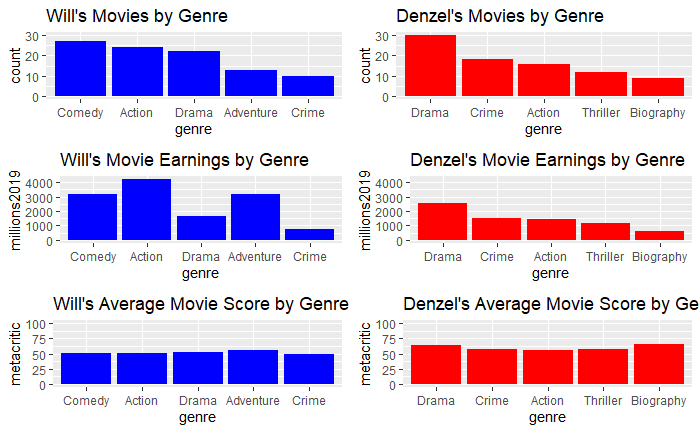
\includegraphics[clip,scale=0.8]{plots/genres.png}
  \caption{\textbf{Movie Genres by Actor}}
  \label{fig:genres}
\end{figure}

By only a cursory glance at the top genres for each actor, we can get a
sense of the differences of their movies. Will Smith's movies are much
more likely to have a lighter tone. The comedy learned from his time in
\emph{The Fresh Prince of Bel-Air} has likely carried over to much of
his other movies. On the other side, Denzel Washington's movies have a
more serious tone. Drama is clearly his top category, with crime being
no more frivolous.

Another interesting point about figure \ref{fig:genres} is the movie
earnings for each genre. Here it is clear that Will's movies have made
much more than Denzel's, but we also can see the variance between the
two. If we look at Denzel's movie earnings by genre, we see that the
earnings scale very similarly to the amount of movies he produces for
each. This could mean that people will consistently see a movie with
Denzel in it irrespective to genre. Whereas, with Will we see that
despite producing many comedy movies, they pale in comparison to his
action movies. Even more significant is that the drama movies he
produces -his third most produced movie genre- lack the commercial
success of his other movies.

The average movie
scores\footnote{Average score here is the average metacritic rating} for
each actor are harder to read, but we can see that Denzel's movies score
higher than Will's for the most part. Will's scores mainly hover in the
low 50s (or mid 50s for adventure) while Denzel are in the high 50s or
low 60s. It is impressive to see that the drama movies made by Denzel
are his second highest rated genre even though they are his most
produced category. I would have thought that the higher quantity of
movies would lead to some flops that bring down the average, but this is
not the case. We can also see that Denzel performs very well in
biographical films. Despite their relatively low commercial success,
they rate as his best genre of the five most that he produces.




%% appendices go here!


\newpage
\theendnotes

%%%%%%%%%%%%%%%%%%%%%%%%%%%%%%%%%%%  biblio %%%%%%%%
\newpage
\begin{auxmulticols}{2}
\singlespacing 
\bibliography{./../../biblio/master.bib}

%%%%%%%%%%%%%%%%%%%%%%%%%%%%%%%%%%%  biblio %%%%%%%%
\end{auxmulticols}

\newpage
{
\hypersetup{linkcolor=black}
\setcounter{tocdepth}{3}
\tableofcontents
}



\end{document}